\section{BranchConnect: The Game}
\label{sec:game}
The online game is accessible by laptops and mobile touch devices, and many users can play at the same time.
The objective of the game is to collect valid layouts of branches which are fabricatable with 3 axis CNC milling machines.
By analyzing the connectivity of branches and target points, the game checks feasibility of a given layout.
Similar to our game, the work \textit{guidance system during furniture design} inspected connectivity, durability, and stability \cite{umetani2012guided}.
Unlike their work, our game puts emphasis on \textit{fabricatability}, as well as \textit{geometric connectivity}, and does not calculate structural performance of each joint.
Instead, we limit valid layout space by selected joint conditions, and group conditions.
We also assume that every fabricated joint works as a rigid joint, thus single connection is counted as stable to hold a pair of branches.


%The workflow of the game is illustrated in Figure~\ref{fig:game_flowchart}.
%\begin{figure}[ht]
%  \begin{center}
%    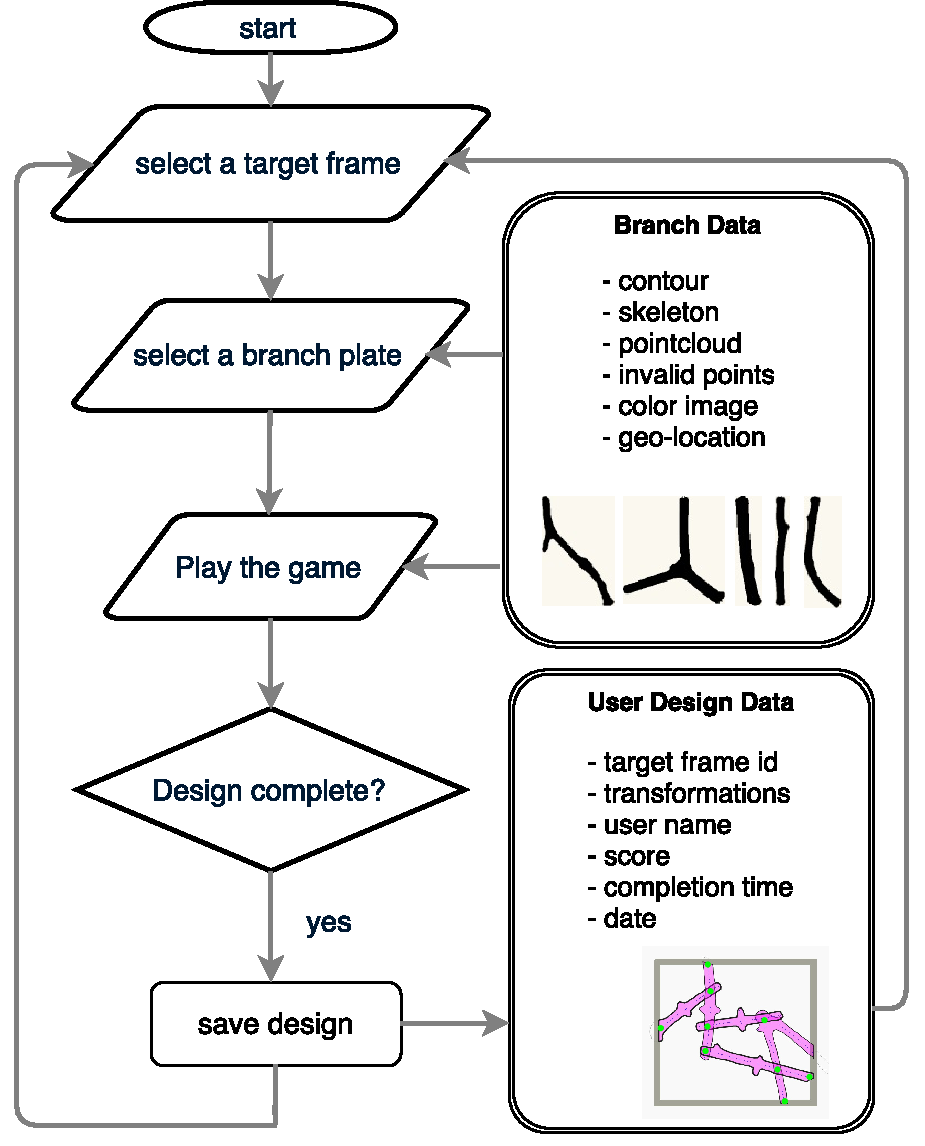
\includegraphics[width = 0.25\paperwidth]{images/system/systemFlowChart.pdf}
%    \caption{The workflow of \textit{BranchConnect}. Branch data and user design data are stored on cloud database.}
%    \label{fig:game_flowchart}
%  \end{center}
%\end{figure}

Firstly a user selects a frame indicating multiple target points to be connected, and then selects a set of branches fixed on a plate (The left in Figure \ref{fig:game_interface}).
After selecting the target frame and the set of branches, the user is guided to the game interface, consisting of the frame with the target points, and the set of available branches (The right in Figure \ref{fig:game_interface}).
The user picks a branch from the available set on the bottom, and then places it in an arbitrary 2D pose through basic manipulations such as move, rotate, and flip.
The number of available branches differs depending on plates.
With the feasible diameter of branches (over 2cm) and the plate size (50cm x 50cm), the number of available branches is most likely up to six.
Within the limited number of branches, the user bridges all the target points by connecting all the used branches in one group.
The game is completed when all the target points are connected.
For higher score, the user can modify the design after the completion, and save it to the database.

\begin{figure}[H]
  \begin{center}
    
\includegraphics[width = 0.4\paperwidth]{images/interface/game_interface.png}
    \caption{Left: the selection interface for target frames (top) and branch panels (bottom). Right: the start interface of the game.}
    \label{fig:game_interface}
  \end{center}
\end{figure}
%
\subsection{Overview}
There are many collision detection libraries available, however, our game needs to detect intersected branch pairs, thus surface contact detection is overkill for our application.
Also most branches come with free-form concave shapes, thus further geometric preparation such as convex decomposition is necessary for using these libraries.
For fast and robust intersection detection, our system extensively uses down-sampled skeletons of branches.

Hubbard and Philip developed collision detection by representing an object with hierarchical 3D spheres aligned on a skeleton \cite{Hubbard:1996:APS:231731.231732}.
Our system takes similar approach but limited in 2D, but more focused on searching fabricatable joints.
In the game, simplified skeletons are used to find the pair of closest skeleton points between two branches.
When a branch is selected, it is counted as an active, and the system searches the closest skeleton point from skeletons of other branches.
More precise joint calculation with higher resolution is further described in the next section.

A joint is created when an intersecting pair is detected, and the pair forms a group.
The group is used for evaluating connections between target points (\textit{Bridged}).
The game is completed once all the target points are connected by a group of branches.
The conditions of joint and group are indicated with simple color-code.
Once the user finishes positioning, score is updated with weighted sum of parameters.
Together with the color-code, the score update guides the user to form a valid design.


\subsection{Joint Condition}
\label{sec:joint}
Joint is the essential entity not only in the game but also in the fabrication process of customized lapped joineries.
Importantly, each pair of branches must have one flipped branch for fabrication constraint.
We describe this further in a later section (see Section \ref{sec:fabrication}).
Figure~\ref{fig:joint_condition} illustrates valid and invalid joint conditions.
Our joint only takes crossed pair (see Figure~\ref{fig:joint_condition}.1) because they are structurally stable, relatively simple to fabricate, and creates diverse designs.
Tangential connections are counted as invalid as fabrication of tangential joinery is challenging with small branches (see Figure~\ref{fig:joint_condition}.3).
A valid joint's angle stays within a fixed range (see Figure~\ref{fig:joint_condition}.1 and 2).
Joints close to metal fixtures are also counted as invalid (see Figure~\ref{fig:joint_condition}.4).
Valid and invalid joints are displayed with green and red respectively.

\begin{figure}[ht]
	\begin{center}
		
\includegraphics[width = 0.4\paperwidth]{images/system/joint_conditions_2.png}
		\caption{Joint conditions. 1. valid joint. 2. invalid for violating the angle. 3. invalid tangential connection. 4. invalid for connecting on a fixture point. }
		\label{fig:joint_condition}
	\end{center}
\end{figure}




To describe the process, we let $\mathcal{B}$ denotes a set of all the available branches, and each branch as $ b_i \in \mathcal{B}$.
While the process checks joint condition through all the branches $\mathcal{B}$, each detected joint is stored in each branch $b_i$, categorized in different conditions such as valid and invalid joints denoted as $j_{\text{valid}, j, i} \in \mathcal{J}_{\text{valid},i}$ and $j_{\text{invalid}, j, i} \in \mathcal{J}_{\text{invalid},i}$ respectively.
When a branch $b_i$ is connected to one of target point $t_j \in \mathcal{T} $, the $t_j$ is stored in $b_i$.


A flowchart of the game system with joint and group conditions is illustrated in Figure \ref{fig:system_flowchart}.

\begin{figure}[ht]
	\begin{center}
		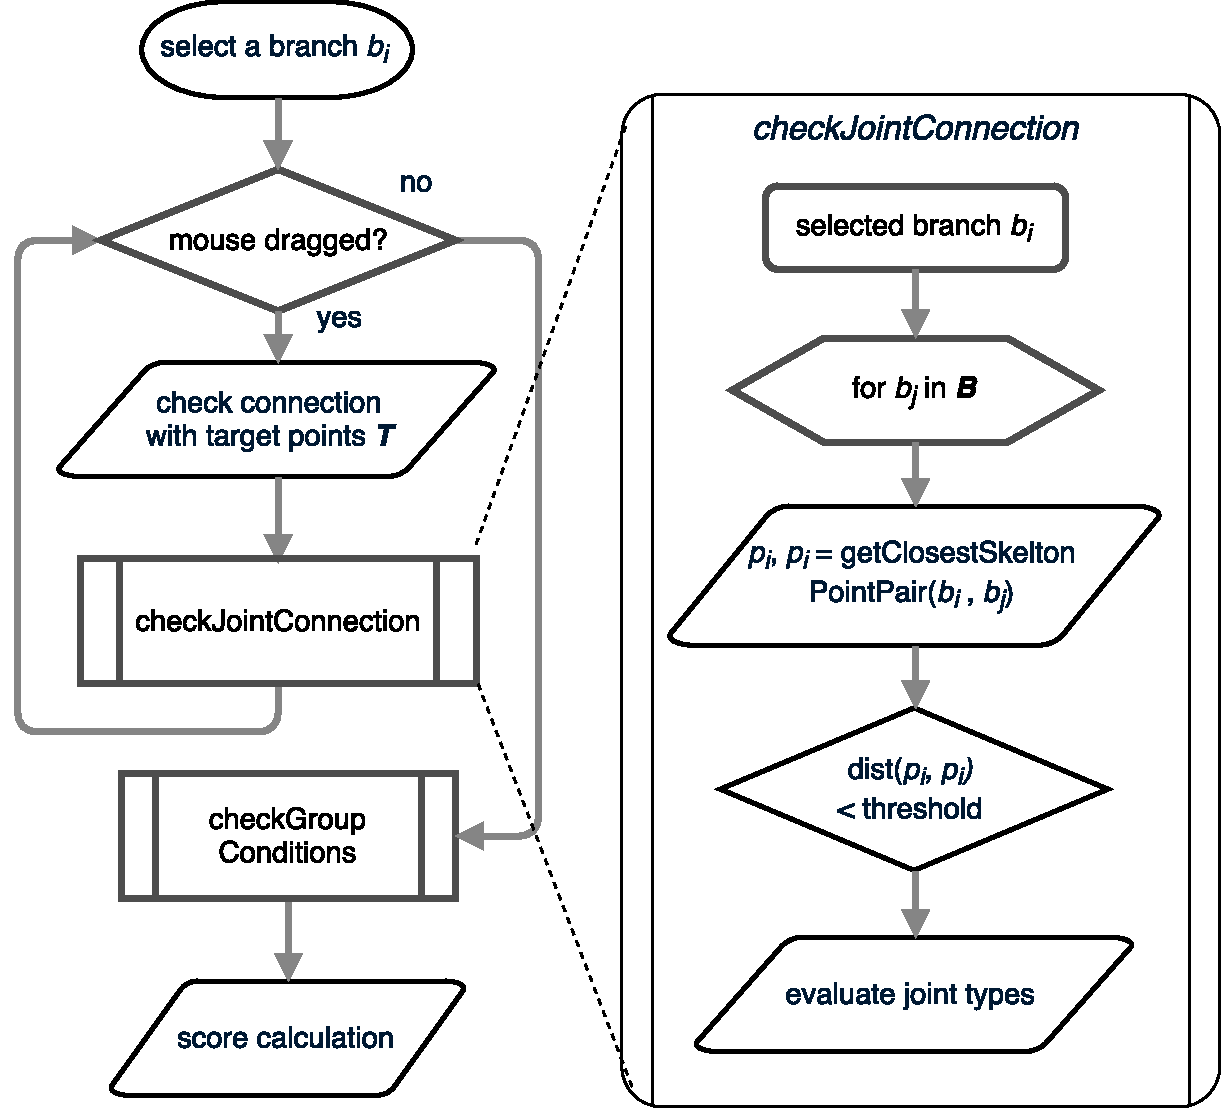
\includegraphics[width = 0.35\paperwidth]{images/system/closestPointAlgorithm.pdf}
		\caption{Left: an overview of the game system with 1.joint checkand 2.group check and 3. score calculation. This process is iteratively executed while a user is exploring layout by dragging a branch. The joint check process is further illustrated in the right, and group condition check is described in Algorithm \ref{al:connection}. }
		\label{fig:system_flowchart}
	\end{center}
\end{figure}

% well as the paired branch $b_{\text{paired},j} \in \mathcal{P}_{\text{paired},i}}$.



\subsection{Group Condition}

After checking joint conditions of all the pairs of branches, the system checks the number of groups as well as its connection with the target points on a frame.
If a group is not connected to any target point nor other groups, the group is \textit{Islanded} and structurally invalid.
While a user is positioning a branch by dragging or rotating, groups are continuously calculated and indicated by simple color (Figure \ref{fig:group}).

\begin{figure}[ht]
  \begin{center}
    
\includegraphics[width = 0.4\paperwidth]{images/interface/groups.jpg}
    \caption{Left: valid group with two target points connected. Middle: valid but three groups. Right: invalid due to the \textit{Islanded} situation. }
    \label{fig:group}
  \end{center}
\end{figure}


After all the joint conditions are checked, we evaluate group conditions.
Through checking the all the branches $\mathcal{B}$, the first group $g_0$ is created and stored as $b_0$.
When a branch is connected to a target point, the graphics of the point changes, and the branch and its belonging group's color also changes.
When a group bridges a pair of target points, a special score is added and displayed in a pop-up square, also the graphics of target point's changes.
The branch connected to the target point is trimmed at the target point, and the trimmed length is subtracted from the score.
%The other paired branch $b_{\text{paired},i}$ stored in $j_{\text{valid}, j}$ is used for tracing the connection with other paired branch in each valid joint $j_i$. \todo{incomplete sentence!}
The game is completed when the number of $\mathcal{G}$ is one, and all the target points are connected with the group.
The algorithm which checks group conditions is described in Algorithm \ref{al:connection}.

\begin{algorithm}
  \caption{Group Condition Update Algorithm}
  \begin{algorithmic}[1]
    \Function{UpdateGroups}{$\mathcal{B}$}
    \State{Reset all the groups $\mathcal{G}$ }
    \State{Create new group $g_0$}
    \State{$b_0 \text{ is added to } g_0$}
    \If{$b_0$ has connected target point $t_i \in \mathcal{T}$}
      \State{$g_0 \text{ sets } t_i$}
    \EndIf
    \State{$g_0 \text{ is added to }  \mathcal{G} $}

    \For{each branch $b_i$ in $\mathcal{B}$}
    \State{\textit{GroupConnection} $\gets false$}
      \For{each group $g_j$ in $\mathcal{G}$}
        \For{each branch $b_j$ in $g_j$}
          \If{ $b_{\text{paired},i} \in \mathcal{P_i}$ has $b_j$}
            \State{ $b_i  \text{ is added to } g_j $}
            \State{ \textit{GroupConnection}  $\gets true$}
            \If{($b_i$ has $t_i$) and ($g_j$ has $t_j$) }
              \State{ Set $g_j$ as \textit{Bridged}}
            \EndIf
            \If{$g_j$ has no $t_j$}
              \State{ Set $g_j$ as \textit{Islanded}}
            \EndIf
            \State {\textit{break}}
          \EndIf
        \EndFor
      \EndFor

      \If{ \textit{GroupConnection} is \textit{false} }
        \State{create new group $g_{new}$}
        \State{ $b_i  \text{ is added to } g_{new}$}
        \State{$g_{new} \text{ is added to }  \mathcal{G}$}
      \EndIf
    \EndFor

  \EndFunction
  \end{algorithmic}
  \label{al:connection}
\end{algorithm}

\subsection{Score Calculation}
In the score calculation processes, follwoing entities forms the score: the numbers of valid and invalid joints on each branch, the number of groups as $N(\mathcal{G} )$, the number of islanded groups as $N(g_{\text{islanded}} \in \mathcal{G} )$, the number of bridged target points as $N(t_{\text{bridged}, i}) \in \mathcal{T} )$.
The trimmed lengths of branches which are connected with target points are denoted as $trimmed(t_j, b_i)$
The score is weighted sum of these joint and group conditions, denoted in Equation (\ref{eq:cost}).
The weights $w_1 \dotso  w_5$ are non-negative weight coefficients pre-adjusted in advance by authors.


\begin{equation} \label{eq:cost}
 \begin{aligned}
 Score =  &\; w_1  \sum_{1}^{N(\mathcal{B})} \sum_{1}^{N(\mathcal{J}_{\text{valid},i})} j_{\text{valid}, j, i}
 + w_2  \sum_{1}^{N(\mathcal{B})} \sum_{1}^{N(\mathcal{J}_{\text{invalid},i})} j_{\text{invalid}, j, i}\\
+ &\; w_3  \sum_{1}^{N(\mathcal{G})} g_{\text{islanded}}
	 + w_4  \sum_{1}^{N(\mathcal{T})} t_{\text{bridged}}
+  w_5 \sum_{1}^{N(\mathcal{T})} trimmed(t_j, b_i)
 \\
   \textrm{s.t.} \; w_j  \geq  &\;0 \; \forall j \in 1, \dotsc , 5
 \end{aligned}
\end{equation}
